\documentclass{article}
\usepackage[utf8]{inputenc}
\usepackage{amsmath}
\usepackage{graphicx}
    \DeclareGraphicsExtensions{.png, .jpeg}
\usepackage{caption}
\usepackage[top=1in, bottom=1in, left=1in, right=1in]{geometry}

\title{STAT 775: Machine Learning \\ HW 02}
\author{Terence Henriod}
\date{\today}

\begin{document}

\clearpage            % All
\maketitle            % this,
\thispagestyle{empty} % removes the page number from the title page

\begin{abstract}
A short implementation and demonstration of na\"{i}ve Bayes classifiers on hand-written digit images.
\end{abstract}

\newpage
\section{Problem Description}
The task: using the \texttt{zipcode} data from the Elements of Statistical Learning book website and Bayes rule, do the following:
\begin{enumerate}
  \item Construct Gaussian classifiers for all of the digits (0-9) using the training data set. Do so by computing the means and covariances of each class in order to fit the Gaussian distribution for the class.
  \item Use the constructed classifiers to classify the test set.
  \item Display the results in a ``confusion matrix."
\end{enumerate}
\textit{Hint}: If you find that a matrix (specifically any of the covariance matrices) is numerically or actually singular, and therefore cannot be inverted, regularize it by adding an identity matrix multiplied by a small factor to ``breathe" on it. This can help make the matrix invertible, but one needs to exercise caution as it can adversely affect the results of computations.

\section{Results}
The na\"{i}ve Bayes classifiers performed rather well, achieving nearly 94\% accuracy. While this does leave something to be desired, improving on this performance benchmark might require improving the numerical accuracy of the program (using something better than double-precision variables), finding a better regularization factor for regularizing non-invertible matrices ($0.5$ seemed to work well enough, no more effort was put forth to improve on this), application of additional techniques (like PCA), or even using this classifier as an element of a composite classifier.

\begin{figure}[h]
  \centering
  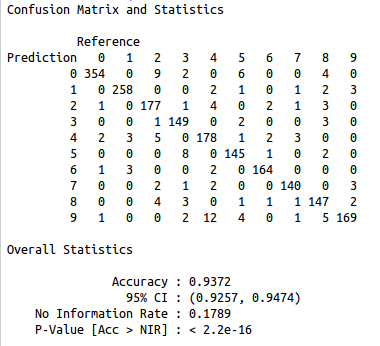
\includegraphics[width=.6\linewidth]{R_confusion_matrix_output}
  \caption{R output of a confusion matrix displaying the classification results using the na\"{i}ve Bayes classifier.}
  \label{fig:confusion_matrix}
\end{figure}

\section{Code}
After struggling for too long with R code and singular matrices, it was deemed better to switch to a familiar and high performance language - namely C++. Thus, the classification code was written in C++ and the confusion matrix was ported to R for data presentation.

\subsection{C++ Code}
\begin{verbatim}
#include <string>
#include <vector>
#include <Eigen/Dense>
#include <cmath>

#include <iostream>
#include <fstream>
#include <exception>

#define PI 3.141592653589793238462643383279502884L
#define REGULARIZATION_FACTOR 0.5

const std::string TRAINING_FILE_NAME = "zip.train"; // 2007 items
const std::string TEST_FILE_NAME = "zip.test"; // 7291 items

typedef struct {
  unsigned label;
  Eigen::VectorXd features;
} ClassificationObject;

typedef struct {
  unsigned label;
  double prior;
  Eigen::VectorXd mean;
  Eigen::MatrixXd covariance;
  double covarianceDeterminant;
  Eigen::MatrixXd covarianceInverse;
} ClassInfo;


std::vector<ClassificationObject>
ReadData(
  const std::string& fileName,
  const unsigned featureDim,
  const unsigned numItems) {

  std::ifstream fin;
  fin.clear(); fin.open(fileName.c_str());

  if (!fin.good()) {
    throw std::exception();
  }

  std::vector<ClassificationObject> data; data.reserve(numItems);

  for (unsigned i = 0; i < numItems; ++i) {
    ClassificationObject classificationObject;
    double dummy;
    fin >> dummy;
    classificationObject.label = (unsigned) dummy;

    classificationObject.features.resize(featureDim);
    for (unsigned j = 0; j < featureDim; ++j) {
      fin >> classificationObject.features(j);
    }
    data.push_back(classificationObject);
  }

  return data;
}

ClassInfo
ComputeClassInfo(
  const std::vector<ClassificationObject>& data,
  const unsigned classLabel,
  const unsigned featureDim) {
 
  ClassInfo classInfo;
  classInfo.label = classLabel;
  classInfo.mean.setZero(featureDim);
  classInfo.covariance.setZero(featureDim, featureDim);

  // compute mean and prior probability at once
  std::vector<ClassificationObject> subset;
  for (const ClassificationObject& classificationObject : data) {
    if (classificationObject.label == classLabel) {
      classInfo.mean += classificationObject.features;
      subset.push_back(classificationObject);
    }
  }
  classInfo.mean /= subset.size();
  classInfo.prior = (double) subset.size() / (double) data.size();

  // covariance matrix
  // Note: I use a nifty trick that is simpler in code (not sure if
  //       simpler computationally). Let $P_i = x_i - mu$, where $i$
  //       corresponds to a particular observation vector. Then
  //       $A$ is the concatenation of all the $P_i$ as column
  //       vectors ($A = [P_1 ... P_m]$). Then
  //       $\frac{1}{m} * A * A^t$ results in the same computations
  //       that create the covariance matrix as more traditional
  //       formulae.
  Eigen::MatrixXd A(featureDim, subset.size());
  for (unsigned j = 0; j < subset.size(); ++j) {
    A.col(j) = subset[j].features - classInfo.mean;
  }
  classInfo.covariance = A * A.transpose();
  classInfo.covariance /= (double) subset.size();
  if (classInfo.covariance.determinant() - 0.1 <= 0.0) {
    Eigen::MatrixXd regularizationMatrix;
    regularizationMatrix.setIdentity(featureDim, featureDim);
    regularizationMatrix *= REGULARIZATION_FACTOR;
    classInfo.covariance += regularizationMatrix;
  }
  classInfo.covarianceDeterminant = classInfo.covariance.determinant();
  classInfo.covarianceInverse = classInfo.covariance.inverse();

  return classInfo;
}

double
GaussianPdf(
  const Eigen::VectorXd& testFeatureVector,
  const ClassInfo& classSummary) {

  const Eigen::VectorXd& x = testFeatureVector;
  const Eigen::VectorXd& mu = classSummary.mean;
  const double& sigmaDet = classSummary.covarianceDeterminant;
  const Eigen::MatrixXd& sigmaInv = classSummary.covarianceInverse; 

  double scalingFactor = 1.0 / sqrt(pow(2.0 * PI, mu.size()) * sigmaDet);
  double exponent = -0.5 * (((x - mu).transpose() * sigmaInv).dot((x - mu)));

  return scalingFactor * exp(exponent);
}

unsigned
ClassifyObject(const ClassificationObject& object, const std::vector<ClassInfo>& classSummaries) {
  unsigned mostLikelyClass = 0;
  double highestProbability = classSummaries.front().label;

  for (const ClassInfo& classSummary : classSummaries) {
    double probability = GaussianPdf(object.features, classSummary) * classSummary.prior;
    if (probability > highestProbability) {
      mostLikelyClass = classSummary.label;
      highestProbability = probability;
    }
  }

  return mostLikelyClass;
}

Eigen::MatrixXi
PerformClassifications(const std::vector<unsigned>& labelSet,
  const std::vector<ClassInfo>& classSummaries,
  const std::vector<ClassificationObject>& testObjects) {

  Eigen::MatrixXi confusionMatrix(labelSet.size(), labelSet.size());
  confusionMatrix.setZero(labelSet.size(), labelSet.size());

  unsigned i = 1;
  unsigned onePercent = testObjects.size() / 100;
  for (const ClassificationObject& object : testObjects) {
    if (i % onePercent == 0) {
      std::cout << i << "% processed." << std::endl;
    }
    i++;

    unsigned classifiedAs = ClassifyObject(object, classSummaries);
    confusionMatrix(object.label, classifiedAs)++;
  }

  return confusionMatrix;
}


int
main(const int argc, const char** argv) {
  std::cout << "Reading Data..." << std::endl;
  std::vector<ClassificationObject> trainingData = ReadData(
    TRAINING_FILE_NAME,
    256,
    7291
  );
  std::vector<ClassificationObject> testData = ReadData(
    TEST_FILE_NAME,
    256,
    2007
  );

  std::cout << "Training Models..." << std::endl;
  std::vector<ClassInfo> classSummaries; classSummaries.reserve(10);
  for (unsigned label = 0; label <= 9; ++label) {
    classSummaries.push_back(ComputeClassInfo(trainingData, label, 256));
  }

  std::cout << "Classifying Objects..." << std::endl;
  Eigen::MatrixXi confusionMatrix = PerformClassifications(
    {0,1,2,3,4,5,6,7,8,9},
    classSummaries,
    testData
  );

  std::cout << "Results:" << std::endl;
  std::cout << confusionMatrix << std::endl;

  return 0;
}
\end{verbatim}

\subsection{R Code}
\begin{verbatim}
############
# Plotting #
############
require(caret)

results <-data.matrix(read.table("results"))
dimnames(results) <- list(c(0,1,2,3,4,5,6,7,8,9), c(0,1,2,3,4,5,6,7,8,9))

actuals.f <- list()
predictions.f <- list()
for (i in 1:nrow(results)) {
  for (j in 1:ncol(results)) {
    actuals.f <- c(actuals.f, rep(i - 1, results[i, j]))
    predictions.f <- c(predictions.f, rep(j - 1, results[i, j]))
  }
}
actuals.f <- factor(unlist(actuals.f))
predictions.f <- factor(unlist(predictions.f))

confusionMatrix(data = predictions.f, reference = actuals.f)
\end{verbatim}

\subsection{The student would like to thank...}
The student would like to thank the authors of the Eigen C++ matrix library. This library has proved quick, easy and effective numerous times, this time being no exception. The Eigen library and more information can both be found at\hfill\\
\texttt{http://eigen.tuxfamily.org}.

\end{document}
